\documentclass{article}
\usepackage[a4paper, margin=20mm]{geometry}
\usepackage{graphicx}
\usepackage{float}
\usepackage{subfigure}
\usepackage{amsmath}
\usepackage{amsfonts}
\title{Practical Submission Sheet}
\newcommand{\bb}[1]{\textbf{#1}}
\newcommand{\ol}[1]{\overline{#1}}
\date{}
\begin{document}
	\maketitle
	\begin{tabular}{ll}
		\bb{Term}: 2020-1 & \bb{Submission Date}: \today\\
		\bb{Lecture Date}: October 9, 2020. & \bb{Practical Number}: 7\\
		\bb{Course Code}: PHY249 & \bb{Section}: G2903\\
		\bb{Registration Number}: 11912610 & \bb{Roll No}: 03\\
		\bb{Student Name}: Aayush Arya & \\
	\end{tabular}
	
	\section*{Aim} To create a logic circuit based on given boolean expressions
	\begin{itemize}
		\item[(i)] $z = [A\cdot (\ol{B} + C) + D]\cdot \bar{B} + C \cdot D$
		\item[(ii)] $ f = x + \ol{x}.\ol{(y+z)} +\ol{y}.(\ol{x} + \ol{z})$
		\item[(iii)] $f =\ol{(\ol{y} + \ol{z})} + y.\ol{z} +  \ol{(x.y)}$ 
	\end{itemize}

	\section*{Concepts Learnt}	
	Realization of boolean expressions using logic gate combinations.
	
	\section*{Key Observations \& Insights}
	Boolean expressions for certain circuits were realized using logic gates, particular using AOI gates. Such complicated circuits can sometimes be avoided by simplifying the expression using either boolean algebra or using K-maps.
	
	\section*{Application Areas}
	Often in electronics one may have to deal with complicated networks, a finger-exercise for dealing with such circuits is beneficial.
	
	\section*{Report}
	For expression (i), an AOI gate combination was simulated as depicted in the figure below.
	\begin{figure}[H]
		\centering
		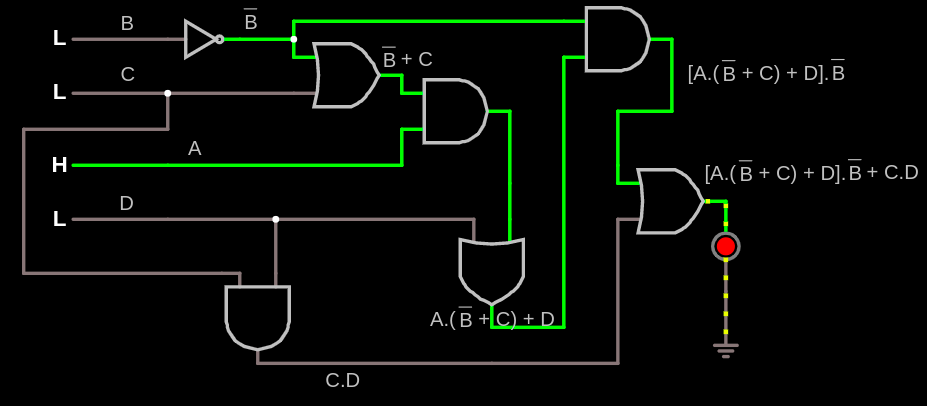
\includegraphics[width=0.75\textwidth]{one}
		\caption{Logic gate combination for the boolean expression (i)}
		\label{circuit1}
	\end{figure}
	 
	The truth table for the boolean function z is then
		\begin{table}[H]
		\centering
		\begin{tabular}{|l|l|l|l|l|}
			\hline
			Input A & Input B & Input C & Input D & Output (z)\\
			\hline
			0 & 0 & 0 & 0 & 1\\
			0 & 0 & 0 & 1 & 1\\
			0 & 0 & 1 & 0 & 1 \\
			0 & 0 & 1 & 1 & 1 \\
			\hline
			0 & 1 & 0 & 0 & 0 \\
			0 & 1 & 0 & 1 & 0\\
			0 & 1 & 1 & 0 & 0\\
			0 & 1 & 1 & 1 & 1\\
			\hline
			1 & 0 & 0 & 0 & 0\\
			1 & 0 & 0 & 1 & 0\\
			1 & 0 & 1 & 0 & 0\\
			1 & 0 & 1 & 1 & 1\\
			\hline
			1 & 1 & 0 & 0 & 0\\
			1 & 1 & 0 & 1 & 0\\
			1 & 1 & 1 & 0 & 0\\
			1 & 1 & 1 & 1 & 1\\
			\hline
		\end{tabular}
		\caption{Truth table for the logic corresponding to the boolean expression $z = [A\cdot (\ol{B} + C) + D]\cdot \bar{B} + C \cdot D$.}
	\end{table}
Expression (ii) can be realised using the following circuit
	\begin{figure}[H]
		\centering
		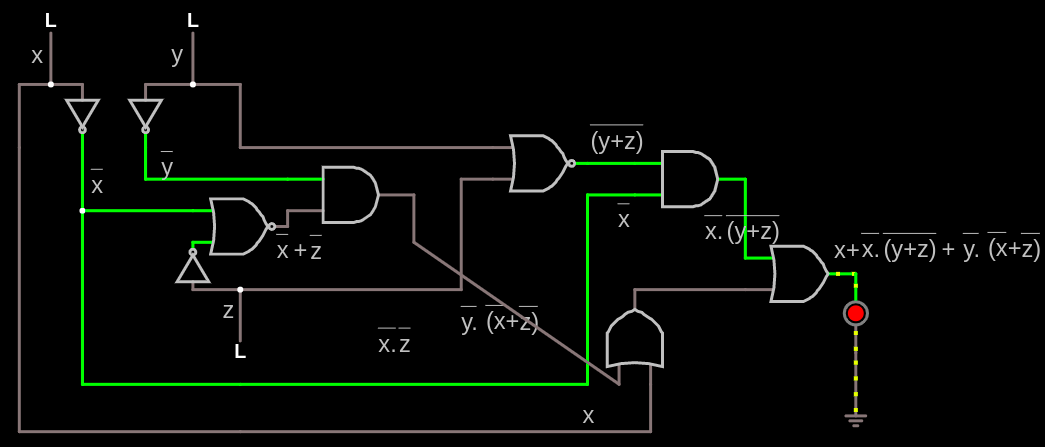
\includegraphics[width=0.75\textwidth]{two}
		\caption{AOI logic circuit corresponding to the expression $ f = x + \ol{x}.\ol{(y+z)} +\ol{y}.(\ol{x} + \ol{z})$ }
		\label{circuit2}
	\end{figure}
	
	The truth table for this logic system is slightly surprisingly 
	
	\begin{table}[H]
	\centering
	\begin{tabular}{|c|c|c|c|}
		\hline
		Input x & Input y & Input x & Output (f)\\
		\hline 
		0 & 0 & 0 & 1\\
		0 & 0 & 1 & 1\\
		0 & 1 & 0 & 1\\
		0 & 1 & 0 & 1\\
		0 & 1 & 1 & 1\\
		1 & 0 & 0 & 1\\
		1 & 0 & 1 & 1\\
		1 & 1 & 0 & 1\\
		1 & 1 & 1 & 1\\
		\hline
	\end{tabular}
	\caption{Truth table for the logic system $ f = x + \ol{x}.\ol{(y+z)} +\ol{y}.(\ol{x} + \ol{z})$.}
\end{table}
 and it can be verified mathematically by reducing the boolean expression, resulting in $f=1$ for all cases.
 
 
For the third and final expression, the boolean logic was realised using the  3 input circuit shown in Figure 3.
 
 	\begin{figure}[H]
 	\centering
 	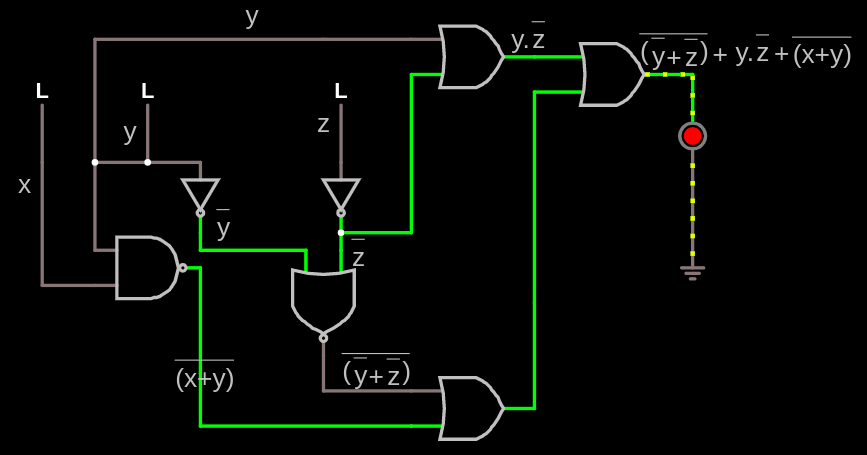
\includegraphics[width=0.75\textwidth]{three}
 	\caption{Circuit diagram for the logic system $f =\ol{(\ol{y} + \ol{z})} + y.\ol{z} +  \ol{(x.y)}$ }
 	\label{circuit3}
 \end{figure}

  Again this expression, when reduced, leads to $f=1$ and thus all output entries in the truth table are $1$, as in table 3.
 
\begin{table}[H]
	\centering
	\begin{tabular}{|c|c|c|c|}
		\hline
		Input x & Input y & Input x & Output (f)\\
		\hline
		0 & 0 & 0 & 1\\
		0 & 0 & 1 & 1\\
		0 & 1 & 0 & 1\\
		0 & 1 & 0 & 1\\
		0 & 1 & 1 & 1\\
		1 & 0 & 0 & 1\\
		1 & 0 & 1 & 1\\
		1 & 1 & 0 & 1\\
		1 & 1 & 1 & 1\\
		\hline
	\end{tabular}
	\caption{Truth table for the logic system $f =\ol{(\ol{y} + \ol{z})} + y.\ol{z} +  \ol{(x.y)}$ .}
\end{table}

\end{document}}